
\documentclass[letterpaper,11pt]{article}

\usepackage{latexsym}
\usepackage{amsmath}
\usepackage{amssymb}
\usepackage{unicode-math}
\usepackage{fancyhdr}
\usepackage[margin=1.0in, left=0.5in, right=0.5in, top=1.25in, headsep=10mm, headheight=15mm]{geometry}
\usepackage{graphicx}

\setmainfont{Latin Modern Roman}
\setmathfont{Latin Modern Math}

\pagestyle{fancy}
\rhead{Mech 222 Mathematics Worksheets\\ Lecture 1, 2}


\newcommand*\limitset[1]{{#1}^\prime}
% Not working in unicode math with xelatex for some reason...
% \newcommand*\closure[1]{\overline #1}
\newcommand*\closureunion[1]{{#1}\cup \limitset{#1}}
\newcommand*\interior[1]{{#1}^\circ}

% Sets of points
% The set of points within some distance #1 from #2
\newcommand*\neighbor[2]{N_{#1}({#2})}
% The neighborhood without #2
\newcommand*\delneighbor[2]{N_{#1}^*({#2})}
\newcommand*\set[1]{\{ #1 \} }
\newcommand*\conjugate[1]{\overline{#1}}
\newcommand*\sequence[2]{\set{#1}_{#2=1}^\infty}
\newcommand*\series[2]{\sum_{#2=1}^\infty #1_{#2}}
\newcommand*\compose[2]{#1 \circ #2}
\newcommand*\udisk{\mathbb{D}}
\newcommand*\disk[2]{D_{#1}(#2)}
\newcommand*\punctdisk[2]{\disk_{ #1 } - \set{#2}}
\newcommand*\complex{\mathbb{C}}
\newcommand*\naturals{\mathbb{N}}
\newcommand{\integers}{\mathbb{Z}}
\newcommand*\rationals{\mathbb{Q}}
\newcommand*\reals{\mathbb{R}}

% Function spaces
\newcommand*\cnfunc[2]{C^{#2}\left(#1 \right)}
\newcommand*\cnfuncdom[1]{C^{#1}\left(\domain \right)}
\newcommand*\linffunc[1]{L^{\infty}\left(#1 \right)}
\newcommand*\linffuncdom{L^{\infty}\left(\domain \right)}
\newcommand*\lnfunc[2]{L^{#2}\left(#1 \right)}
\newcommand*\lnfuncdom[1]{L^{#1}\left(\domain \right)}
\newcommand*\sobolev[3]{W^{#2, #3}\left(#1 \right)}
\newcommand*\sobolevdom[2]{W^{#1, #2}\left(\domain \right)}
\newcommand*\sobolevh[2]{H^{#2}\left(#1 \right)}
\newcommand*\sobolevhdom[1]{H^{#1}\left(\domain \right)}
\newcommand*\sobolevcs[3]{W_0^{#2, #3}\left(#1 \right)}
\newcommand*\sobolevcsdom[2]{W_0^{#1, #2}\left(\domain \right)}
\newcommand*\sobolevhcs[2]{H_0^{#2}\left(#1 \right)}
\newcommand*\sobolevhcsdom[1]{H_0^{#1}\left(\domain \right)}

\newcommand*\grad{D}
\newcommand*\graddir[1]{D_{#1}}
\newcommand*\lapl{∆}
\newcommand*\diffquot[1]{D^{#1}}
\newcommand*\diffquotdir[2]{D_{#2}^{#1}}

\newcommand*\domain{U}
\newcommand*\bndry[1]{\partial #1}
\newcommand*\bndrydom{\partial \domain}
\newcommand*\compactcont{\subset \subset} % U \compactcont V \rightarrow U \subset \closure{U} \subset V, where U, V are (open) domains

\newcommand*\ballunit{B_1}
\newcommand*\ball[2]{B_{#2}(#1)}
\newcommand*\bunitsurfarea[1]{\omega_{#1}}
\newcommand*\bunitsurfareadef{\omega_n}
\newcommand*\bunitvolume[1]{\alpha_{#1}}
\newcommand*\bunitvolumedef{\alpha_n}

\newcommand*\limitto[2]{\lim \limits_{#1 \rightarrow #2}}

\newcommand{\dd}[1]{\;\mathrm{d}#1}
\newcommand{\dx}{\dd{x}}
\newcommand{\dy}{\dd{y}}
\newcommand{\dz}{\dd{z}}
\newcommand{\dr}{\dd{r}}
\newcommand{\ds}{\dd{s}}
\newcommand{\dS}{\dd{S}}
\newcommand{\dt}{\dd{t}}
\newcommand*\pderiv[2]{\frac{\partial #1}{\partial #2}}
\newcommand*\nthpderiv[3]{\frac{\partial^{#3} #1}{\partial #2^{#3}}}
\newcommand*\deriv[2]{\frac{\dd{#1}}{\dd{#2}}}
\newcommand*\nthderiv[3]{\frac{\dd{^{#3} #1}}{\dd{#2^{#3}}}}

% Norms
\newcommand*\linfnorm[2]{\left\lVert#1\right\rVert_{L^{\infty}(#2)}}
\newcommand*\linfnormdom[1]{\left\lVert#1\right\rVert_{L^{\infty}(\domain)}}

\newcommand*\lnorm[3]{\left\lVert#1\right\rVert_{L^{#2}(#3)}}
\newcommand*\lnormdom[2]{\left\lVert#1\right\rVert_{L^{#2}(\domain)}}

\newcommand*\hnorm[3]{\left\lVert#1\right\rVert_{H^{#2}(#3)}}
\newcommand*\hnormdom[2]{\left\lVert#1\right\rVert_{H^{#2}(\domain)}}

\newcommand*\wnorm[4]{\left\lVert#1\right\rVert_{W^{#2, #3}(#4)}}
\newcommand*\wnormdom[3]{\left\lVert#1\right\rVert_{W^{#2, #3}(\domain)}}

\DeclareMathOperator{\res}{res}
\DeclareMathOperator{\sign}{sign}
\DeclareMathOperator{\diam}{diam}
\DeclareMathOperator{\partition}{Partition}

% Matrix computations
\newcommand*\trace[1]{\text{tr}\left( #1 \right)}

% Average integral from https://tex.stackexchange.com/questions/759/average-integral-symbol
\def\Xint#1{\mathchoice
{\XXint\displaystyle\textstyle{#1}}%
{\XXint\textstyle\scriptstyle{#1}}%
{\XXint\scriptstyle\scriptscriptstyle{#1}}%
{\XXint\scriptscriptstyle\scriptscriptstyle{#1}}%
\!\int}
\def\XXint#1#2#3{{\setbox0=\hbox{$#1{#2#3}{\int}$ }
\vcenter{\hbox{$#2#3$ }}\kern-.6\wd0}}
\def\ddashint{\Xint=}
\def\dashint{\Xint-}
\def\avgint{\dashint}


\begin{document}
\section*{Integration Review - Substitution, Integration by Parts}
  \subsection*{Problems}
  Compute the following integrals:
  \begin{enumerate}
    \item $\int \limits_{0}^{\pi / 4} e^{\tan(x) + 1} \sec^2(x) \dx$\\
      \newline
      \newline

    \item $\int \limits_{0}^{\pi / 4} e^{\tan(x) + y} \sec^2(x) \dx$\\
      \newline
      \newline

    \item $\int \limits_{0}^{1} e^{\tan(x) + y} \dy$\\
      \newline
      \newline

    \item $\int \limits_{0}^{1} x e^{x} + y \dx$\\
      \newline
      \newline

    \item Challenge: $\int \limits_{0}^{1} x^2 y^{x} \dx$\\
      \newline
      \newline
  \end{enumerate}

\section*{Iterated Integrals}
  Recall that to evaluate $\int \limits_{a}^{b} \int \limits_{c}^{d} f(x, y) \dx \dy$,
  we can just compute $g(y) = \int \limits_{c}^{d} f(x, y) \dx$ with constant $y$,
  and then the solution is $\int \limits_{a}^{b} g(y) \dy$.

  \subsection*{Example}
  \begin{align*}
    & \int \limits_{0}^{1} \int \limits_{0}^{2} e^{x} y^2 \dx \dy\\
    & g(y) = \int \limits_{0}^{2} e^{x} y^2 + 1 \dx = e^x y^2 + x \bigg \rvert_{x = 0}^{2} = (e^{2} - e^{0}) y^2 + (2 - 0)
  \end{align*}
  Then
  \begin{align*}
    & \int \limits_{0}^{1} \int \limits_{0}^{2} e^{x} y^2 \dx \dy = \int \limits_{0}^{1} g(y) \dy\\
    & = \int \limits_{0}^{1} (e^{2} - 1) y^2 + 2 \dy
      = \frac{1}{3} (e^{2} - 1) y^3 + 2 y \bigg \rvert_{y = 0}^{1}
      = \frac{1}{3} (e^{2} - 1) + 2
  \end{align*}

  Frequently, the domain of integration will need to be determined, either from a geometric description or a picture.
  For example, the domain of integration for the example is a rectangle with a corner at the origin and at the point $(2, 1)$.
  \begin{figure}[h]
    \centering 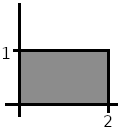
\includegraphics{mech222/lecture_1a_example_domain.png}
    \caption{A picture of the domain}
  \end{figure}
  Recall that the process for computing the iterated integrals is as follows:
  \begin{enumerate}
    \item Convert the region of integration into a an upper and lower bound for one variable in terms of the other(s).
      This may be a piecewise function that needs to be split into multiple integrals.
      These bounds will be used for the inner integral; note that they can only depend on the variables integrated in the outer integral(s).
    \item Compute the inner integral, holding the other variables constant.
      By convention, the inner integral is over the first differential variable, ie
      $\int \limits_{a}^{b} \int \limits_{c(y)}^{d(y)} \int \limits_{e(x, y)}^{f(x, y)} g(x, y, z) \dz \dx \dy$
      the inner integral would be over $z$.
    \item Substitute in the upper and lower bounds, and repeat the integration over the next variable.\\
      $\int \limits_{a}^{b} \int \limits_{c(y)}^{d(y)} \int \limits_{e(x, y)}^{f(x, y)} g(x, y, z) \dz \dx \dy$
      would integrate over $x$ next, and then finish with $y$.
  \end{enumerate}
  \subsection*{Problems}
  Compute the following iterated integrals.

  \begin{enumerate}
    \item $\int \limits_{0}^{1} \int \limits_{2}^{4} x e^{x} + y \dy \dx$\\
      \newline
      \newline
      \newline
    \item $\int \limits_{2}^{4} \int \limits_{0}^{1} x e^{x} + y \dx \dy$\\
      (This result is not a coincidence; it is an example of Fubini's theorem)\\
      \newline
      \newline
      \newline
    \item $\int \limits_{0}^{1} \int \limits_{x}^{2 x} 5 x \dy \dx$\\
      \newline
      \newline
      \newline
    \item $\int \limits_{0}^{1} \int \limits_{0}^{e^{x}} \sin(e^x) \dy \dx$\\
      \newline
      \newline
      \newline
    \item Integrate $f(x, y) = x^2 + 2 x y$ over the area with boundaries at $x = 0$, $x = 1$, $y = 0$, $y = x$.\\
      \newline
      \newline
      \newline
    \item Integrate $f(x, y) = \cos(x) y^{2} + y$ over the right triangle with vertices at the points $(0, 0)$, $(1, 0)$, and $(0, 1)$.\\
      \newline
      \newline
      \newline
    \item Integrate $f(x, y) = 3 x^2 \sqrt{1 - y^2}$ over the unit circle centered at the origin.\\
      Hint: Integrate over $x$ first\\
      \newline
      \newline
      \newline
    \item Integrate $f(x, y) = 1$ over the unit circle centered at the origin.\\
      Hint: Use a trigonometric substitution for the outer integral, and then apply trigonometric identities.\\
      \newpage
    \item Challenge $\int \limits_{0}^{1} \int \limits_{x}^{1} \sin(y^2) \dy \dx$\\
      Hint: Try drawing the region and deducing bounds for this integral with $x$ as the inner term.
      ie, convert this integral to the form $\int \limits_{a}^{b} \int \limits_{c(y)}^{d(y)} \sin(y^2) \dx \dy$.\\
      \newline
      \newline
      \newline
  \end{enumerate}
\end{document}
